\documentclass[titlepage, a4paper]{article}
\usepackage[swedish]{babel}
\usepackage[utf8]{inputenc}
\usepackage{color}
\usepackage{graphicx}
\usepackage{etoolbox}
\usepackage{stringenc}
\usepackage{pdfescape}

% Sidformat
\usepackage{a4wide}

% Fixa Appendix-titlar
\usepackage[titletoc,title]{appendix}

% Bättre tabeller
\usepackage{tabularx}

% Bättre bildtexter
\usepackage[margin=10pt,font=small,labelfont=bf,labelsep=endash]{caption}

% Enkelt kommando som låter mig attgöra-markera text
\newcommand{\todo}[1] {\textbf{\textcolor{red}{#1}}}

% Nytt \paragraph låter oss ha onumrerade bitar
\makeatletter
\renewcommand\paragraph{\@startsection{paragraph}{4}{\z@}%
{-3.25ex\@plus -1ex \@minus -.2ex}%
{1.5ex \@plus .2ex}%
{\normalfont\normalsize\bfseries}}
\makeatother

\providecommand{\LIPSlogga}{../mall/logga1.png}
\providecommand{\LIPSdatum}{\today}

%% Headers och Footers
\usepackage{fancyhdr}
\pagestyle{fancy}
\lhead{\includegraphics[scale=0.4]{\LIPSlogga}}
\rhead{\ifdef{\LIPSutfardare}{Utfärdat av \LIPSutfardare \\\LIPSdatum}\LIPSdatum}
\lfoot{\LIPSkursnamn \\ \LIPSdokumenttyp}
\cfoot{\thepage}
\rfoot{\LIPSprojektgrupp \\ \LIPSprojektnamn}

%% Titelsida
\newcommand{\LIPSTitelsida}{%
{\ }\vspace{45mm}
\begin{center}
  \textbf{\Huge \LIPSdokument}
\end{center}
\begin{center}
  {\Large Redaktör: \LIPSredaktor}
\end{center}
\begin{center}
  {\Large \textbf{Version \LIPSversion}}
\end{center}
\vfill
\begin{center}
  {\large Status}\\[1.5ex]
  \begin{tabular}{|*{3}{p{40mm}|}}
    \hline
    Granskad & \LIPSgranskare & \LIPSgranskatdatum \\
    \hline
    Godkänd & \LIPSgodkannare & \LIPSgodkantdatum \\
    \hline
  \end{tabular}
\end{center}
\newpage
}

% Projektidentitet
\newenvironment{LIPSprojektidentitet}{%
{\ }\vspace{45mm}
\begin{center}
  {\Large PROJEKTIDENTITET}\\[0.5ex]
  {\small
  \LIPSartaltermin, \LIPSprojektgrupp\\
  Linköpings Tekniska Högskola, IDA
  }
\end{center}
\begin{center}
  {\normalsize Gruppdeltagare}\\
  \begin{tabular}{|l|l|p{25mm}|l|}
    \hline
    \textbf{Namn} & \textbf{Ansvar} & \textbf{Telefon} & \textbf{E-post} \\
    \hline
}%
{%
    \hline
  \end{tabular}
\end{center}
\begin{center}
  {\small
    \ifdef{\LIPSgruppadress}{\textbf{E-postlista för hela gruppen}: \LIPSgruppadress\\}{}
    \ifdef{\LIPSgrupphemsida}{\textbf{Hemsida}: \LIPSgrupphemsida\\[1ex]}{}
    \ifdef{\LIPSkund}{\textbf{Kund}: \LIPSkund\\}{}
    \ifdef{\LIPSkundkontakt}{\textbf{Kontaktperson hos kund}: \LIPSkundkontakt\\}{}
    \ifdef{\LIPSkursansvarig}{\textbf{Kursansvarig}: \LIPSkursansvarig\\}{}
    \ifdef{\LIPShandledare}{\textbf{Handledare}: \LIPShandledare\\}{}
  }
\end{center}
\newpage
}
\newcommand{\LIPSgruppmedlem}[4]{\hline {#1} & {#2} & {#3} & {#4} \\}

%% Dokumenthistorik
\newenvironment{LIPSdokumenthistorik}{%
\begin{center}
  Dokumenthistorik\\[1ex]
  %\begin{small}
    \begin{tabular}{|l|l|p{60mm}|l|l|}
      \hline
      \textbf{Version} & \textbf{Datum} & \textbf{Utförda förändringar} & \textbf{Utförda av} & \textbf{Granskad} \\
      }%
    {%
			\hline
    \end{tabular}
  %\end{small}
\end{center}
}

\newcommand{\LIPSversionsinfo}[5]{\hline {#1} & {#2} & {#3} & {#4} & {#5} \\}

% Kravlistor
\newenvironment{LIPSkravlista}{
	\center
		\tabularx{\textwidth}{| p{1.2cm} | p{1.9cm} | X | c |}
			\hline
			\textbf{Krav} & \textbf{Förändring} & \textbf{Beskrivning} & \textbf{Prioritet} \\\hline
}
{
		\endtabularx
	\endcenter
}

\newcounter{LIPSkravnummer}
\addtocounter{LIPSkravnummer}{1}
\newcommand{\LIPSkrav}[4][Krav \arabic{LIPSkravnummer}]{{#1} & {#2} & {#3} & {#4} \stepcounter{LIPSkravnummer}\\\hline}


% Leveranskravlistor
\newenvironment{LIPSleveranskravlista}{
	\center
		\tabularx{\textwidth}{| p{1.2cm} | p{1.9cm} | X | X |}
			\hline
			\textbf{Krav} & \textbf{Förändring} & \textbf{Beskrivning} & \textbf{Deadline}\\\hline
}
{
		\endtabularx
	\endcenter
}

\newcounter{LIPSleveranskravnummer}
\addtocounter{LIPSleveranskravnummer}{1}
\newcommand{\LIPSleveranskrav}[4][Krav \arabic{LIPSkravnummer}]{{#1} & {#2} & {#3} & {#4} \stepcounter{LIPSkravnummer}\\\hline}


% Milstolps-lista
\newenvironment{LIPSmilstolpar}{
	\center
		\tabularx{\textwidth}{| p{1.2cm} | X | l |}
			\hline
			\textbf{Nr} & \textbf{Beskrivning} & \textbf{Datum} \\\hline
}
{
		\endtabularx
	\endcenter
}

\newcounter{LIPSstolpnummer}
\addtocounter{LIPSstolpnummer}{1}
%\newcommand{\LIPSmilstolpe}[3][Krav \arabic{LIPSstolpnummer}]{{#1} & {#2} & {#3} \stepcounter{LIPSstolpnummer}\\\hline}
\newcommand{\LIPSmilstolpe}[3]{{#1} & {#2} & {#3} \\\hline}

% Aktivitets-lista
\newenvironment{LIPSaktivitetslista}{
	\center
		\tabularx{\textwidth}{| p{0.3cm} | X | c | c | c |}
			\hline
			\textbf{Nr} & \textbf{Beskrivning} & \textbf{Beroende av} & \textbf{Timmar} & \textbf{datum} \\\hline
}
{
		\endtabularx
	\endcenter
}

\newcounter{LIPSaktivitetsnummer}
\addtocounter{LIPSaktivitetsnummer}{1}
% \newcommand{\LIPSaktivitet}[4][\arabic{LIPSstolpnummer}]{{#1} & {#2} & {#3} & {#4} \stepcounter{LIPSstolpnummer}\\\hline}
\newcommand{\LIPSaktivitet}[5]{{#1} & {#2} & {#3} & {#4} & {#5}\\\hline}

% Mall för mötesprotokoll
\newenvironment{projektmote}[2]{
  {\ }\vspace{5mm}

  \centerline{\textbf{\Huge #1}}
  \vspace{2mm}
  \centerline{\LARGE #2}
  \vspace{10mm}

  \begin{itemize}
}
{
  \end{itemize}
}

\newcounter{paragrafnummer}
\addtocounter{paragrafnummer}{1}
\newcommand{\paragraf}[1]{\item{\textsection \arabic{paragrafnummer}. {#1}}\addtocounter{paragrafnummer}{1}}

% Mall för Statusrapport
\newenvironment{statusrapport}{
  \center
    \tabularx{\textwidth}{| p{0.4cm} | X | X | p{14.5mm} | p{13.5mm} | p{16.5mm} | p{16.5mm} |}
    \hline
    \textbf{Nr} & \textbf{Aktivitet} & \textbf{Beroenden} & \textbf{Planerad tid} & \textbf{Nedlagd tid} & \textbf{Planerad klar} & \textbf{Beräknat klart} \\\hline
}
{
    \endtabularx
  \endcenter
}

\newcommand{\aktivitetstatus}[7]{{#1} & {#2} & {#3} & {#4} & {#5} & {#6} & {#7} \\\hline}	% Importera generella layout-strukturer

% Information nödvändig för generella layout-strukturer
\newcommand{\LIPSredaktor}{Johan Isaksson}
\newcommand{\LIPSversion}{0.1}
\newcommand{\LIPSdokument}{Testrapport 2}
\newcommand{\LIPSdokumenttyp}{Testrapport}
\newcommand{\LIPSgranskatdatum}{-}
\newcommand{\LIPSgranskare}{Andreas Runfalk}
\newcommand{\LIPSgodkannare}{Andreas Runfalk}
\newcommand{\LIPSgodkantdatum}{-}
\newcommand{\LIPSkursnamn}{TDDD77}
\newcommand{\LIPSprojektnamn}{Prediktionsreglering}
\newcommand{\LIPSprojektgrupp}{Grupp 2}
%\newcommand{\LIPSgruppadress}{\todo{Ta bort}}
\newcommand{\LIPSartaltermin}{VT, 2015}
\newcommand{\LIPSgrupphemsida}{http://pum-2.ida.liu.se/}
\newcommand{\LIPSkund}{SAAB}
\newcommand{\LIPSkundkontakt}{Daniel Simon}
\newcommand{\LIPSkursansvarig}{Kristian Sandahl}
\newcommand{\LIPShandledare}{Andreas Runfalk}

% Dokument-specifika paket
\usepackage{tabularx}
\usepackage{pdfpages}
\usepackage{tikz}
\usepackage{graphicx}
\usetikzlibrary{shapes, arrows}

\pagenumbering{roman}


\DeclareGraphicsRule{.0.pdf}{pdf}{*}{}

\begin{document}

\LIPSTitelsida

\begin{LIPSprojektidentitet}
	\LIPSgruppmedlem{Adam Sestorp}{Team leader}{070 9987270}{adase035@student.liu.se}
	\LIPSgruppmedlem{Dennis Ljung}{Dokumentansvarig}{070 8568148}{denlj069@student.liu.se}
	\LIPSgruppmedlem{Alexander Yngve}{Utvecklingsansvarig}{076 2749762}{aleyn573@student.liu.se}
	\LIPSgruppmedlem{Martin Söderén}{Analysansvarig}{070 8163241}{marso329@student.liu.se}
	\LIPSgruppmedlem{Ruben Das}{Kvalitetssamordnare}{073 7355892}{rubda680@student.liu.se}
	\LIPSgruppmedlem{Sebastian Fast}{Arkitekt}{073 3885208}{sebfa861@student.liu.se}
	\LIPSgruppmedlem{Johan Isaksson}{Testledare}{070 2688785}{johis024@student.liu.se}
\end{LIPSprojektidentitet}

\newpage
\tableofcontents	%Innehållsförteckning
%\listoffigures
%\listoftables

%\newpage

%\begin{LIPSdokumenthistorik}
%\LIPSversionsinfo{0.1}{2015-03-05}{Första utkast}{Johan Isaksson}{}
%\end{LIPSdokumenthistorik}

\newpage
\pagenumbering{arabic}	%Påbörja sidnumrering

% Inledning, översikt osv


\section{Inledning}
Denna rapport redovisar de test som utförts och skapats under iteration 2 i projektet. I första delen beskrivs hur testproceduren gått till samt vilka som delatagit. Sedan efter det beskrivs de objekt som har testats.
\subsection{Deltagare}
Genom hela iteration 2 har samtliga gruppmedlemmar jobbat med testning. Johan, Alexander och Ruben har fortsatt testandet av lösaren, Martin har fortsatt testa ny kod i matrisbiblioteket, Adam har testat ny funktionalitet i parsern, och Dennis och Sebastian har jobbat med integrationen mot matlab där test av matrisomvandligar har krävts. 

\subsection{Procedur}
Under iteration 2 har fler delar integrerats med varandra, till exempel som att lösaren har kopplats ihop med matlab. Detta har lett till att projektmedlemmarna jobbat mer tillsammans och på ett effektivare sätt kunnat testa koden. Testen har fortfarande bestått utav Black-Box-test, men denna gång varit mer övergripande. Här är ett exempel på ett test utav lösaren:

$$quadopt\_solver(problem);$$
$$assert(compare\_matrices(problem\rightarrow solution, expected\_ans));$$

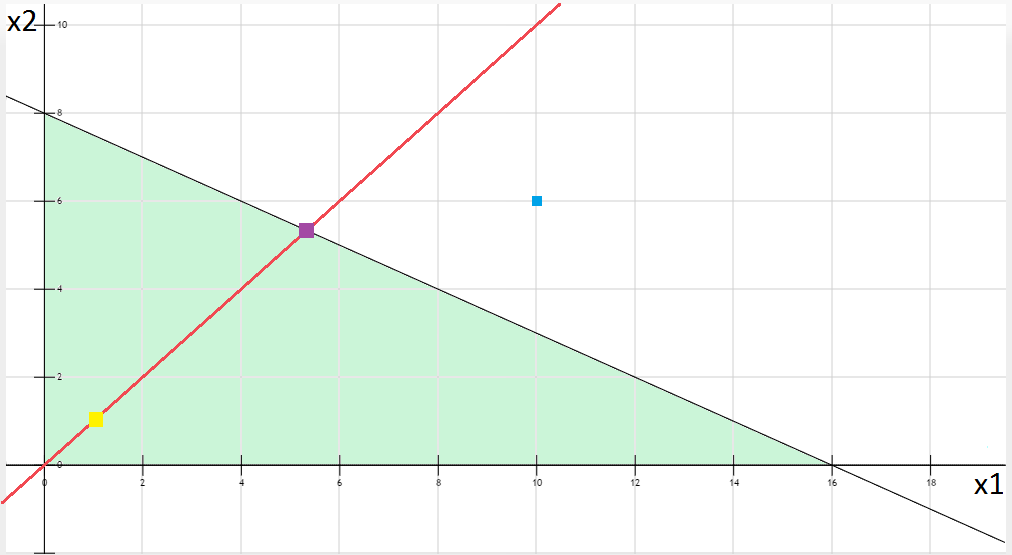
\includegraphics[scale=0.6]{grafik/prob.png}


\raggedright I bilden ovan är det gröna området det tillåtna rummet som spänns upp utav ''$\geq$''-bivillkoren. Det röda sträcket är ett ''$=$''-bivillkor (alltså ett bivillkor där punkten måste ligga på linjen). Den blåa pricken är målfunktionens globala minimum, den gula pricken är startpunkten och den lila är optimum. \newline
Om problemet är som beskrivet i bilden ovan, så skulle variabeln ''problem'' beskriva hela problemet, och ''expected\_ans'' vara den förväntade optimala punkten (lila pricken). Om asserten misslyckas betyder det att lösaren inte lyckades lösa problemet.



\section{Tester}
Av följande objekt och funktioner har tester skapats och utförts i iteration 1:

\subsection{Status}
Här visas teststatus för de olika delarna.
\begin{itemize}
\item{Matrisbibliotek - 90\%}
\item{Lösare av linjära system - 95\%}
\item{Lagrangemultiplikatorberäknare - 100\%}
\item{Stegberäknare - 100\%}
\item{Strukturen work\underline{\space}set - 100\%}
\item{Byggsystem - 95 \%}
\item{GUI och parser - 55\%}
\item{Lösare - 80\%}
\end{itemize}
\raggedright Procentsatsen kan ses som ett uppskattat mått på hur tillförlitlig koden är just nu. Detta eftersom mycket kod tros fungera men ej testats tillräckligt. 

\newpage
\subsection{Slutfört}
Som man kan se ovan är testning utav tre delar klar, Lagrangemultiplikatorer, Stegberäknare och work\_set. Lagrange- och stegdelen var relativt små delar och deras uppgifter var otvetydliga. Däremot så var svårare att avgöra hur komplett work\_set var. Anledningen till att den är satt till 100\% är då lösaren inte behöver mer funktionalitet från work\_set än vad som finns just nu. Dock finns det än risk att ytterligare funktioner kan tillkomma i framtiden, men de är i så fall av låg prioritet. 

\subsection{Pågående}
Just nu testas lösaren för fullt, detta genom att jämföra lösarens svar från olika problem med svar från matlabs egna funktioner. \newline
Test av Parsern har kommit igång, men den är långt ifrån komplett då definitionerna av parserns uppgifter fortfarande är ganska vaga. \newline 
Olika delar av matrisbiblioteket håller fortfarande på att testas. 

\subsection{Kommande}
Det som ska testas i framtiden är de resterande funktionerna i varje del. Men mestadels funktioner till optimeringslösaren för att garantera dens pålitlighet. Just nu är de färdiga funktionerna testade med ganska små datamängder. Detta då vi vet vad produkten ska användas till. Men skalbarheten hos olika funktioner måste testas då problemet eventuellt byggs ut och programmet måste kunna hantera stora matriser. Under iteration 2 ska GUI:t och parsern börja implementeras och då kommer test av dessa krävas i större utsträckning.


\end{document}
